\chapter{Results}
\label{chap:Results}
The Docker containers, running on an \textit{HP ProLiant DL380p Gen8} server with \textit{32 cores} at \textit{2.70 GHz} and \textit{175.97 GB of RAM}, were configured to execute AFLNet, ChatAFL, and various Fallaway configurations for 24 hours, sharing the same resources.
\\After 24h of fuzzing, we can look at the results and analyze them, but before this, another step has been done to obtain the coverage of AFLNet and ChatAFL. By default, the output of AFLNet and ChatAFL is a \textit{gcov} file, giving line and branch coverage.
\\Using the \textbf{replayer} (a component designed to replay test cases or inputs, generating a coverage report), we have replicated the queue of AFLNet and ChatAFL and replayed it to calculate the complete coverage.
\\In Table \ref{tab:fuzzer_comparison} we can see the comparison of the coverage and total executions for Fallaway, AFLNet, and ChatAFL. 
\\Fallaway has been run with different loop configuration (this is explicited by the number after \textit{``Fallaway"} in the table). The strategy used is the \textit{mcsm-oe} (\textit{Multiple Corpus Single Map - Outgoing Edges}), because it has shown to be better than the other strategies \cite{Fallaway}.
\\There are also other two columns, \textit{``$>$ AFLNet"} and \textit{``$>$ ChatAFL"}, that show the time in which the fuzzer overcame the coverage of that column's fuzzer.
\\In bold we are highlighting:
\begin{itemize}
    \item The highest and lowest coverage.
    \item The highest and lowest time to overcome AFLNet.
    \item The highest and lowest time to overcome ChatAFL.
    \item The highest and lowest number of total executions.
\end{itemize}

\section{Fuzzer Analysis}

\begin{table}[H]
    \centering
    \resizebox{1\textwidth}{!}{
    \begin{tabular}{|c|c|c|c|c|}
    \hline
    \textbf{Fuzzer} & \textbf{Complete Coverage} & \textbf{$>$ AFLNet} & \textbf{$>$ ChatAFL} & \textbf{Total Executions *} \\
    \hline
    Fallaway 2000 & \textbf{5.96\% (905/15168)} & 2h 56m 24s & \textbf{6h 25m 48s} & \textbf{120,726,564} \\
    \hline
    Fallaway 1000 & 5.82\% (883/15168) & 3h 22m 48s & 3h 35m 24s & 79,987,763 \\
    \hline
    Fallaway 500 & 5.88\% (893/15168) & \textbf{0h 45m 23s} & \textbf{1h 48m 0s} & 81,231,325 \\
    \hline
    Fallaway 250 & 5.87\% (891/15168) & 0h 51m 16s & 2h 9m 0s & 96,929,952 \\
    \hline
    Fallaway 100 & 5.91\% (896/15168) & 4h 17m 24s & 4h 43m 48s & 59,916,978 \\
    \hline
    Fallaway 10 & \textbf{4.89\% (741/15168)} & Nan & Nan & 18,892,551 \\
    \hline
    AFLNet & 5.47\% (830/15168) & Nan & Nan & \textbf{209,776} \\
    \hline
    ChatAFL & 5.60\% (850/15168) & \textbf{9h 16m 48s} & Nan & 241,242 \\
    \hline
    \end{tabular}
    }
    \caption{Comparison of Coverage and Total Executions for Fallaway, AFLNet, and ChatAFL (Fallaway has been run with different loop values).\\ \textbf{*} Take a look at Section \ref{sec:fallaway_analysis} for a deep understanding of this value.}
    \label{tab:fuzzer_comparison}
\end{table}

\section{Coverage Analysis Over Time and Configurations}

In the next figures, we can see the coverage of the three fuzzers over time.
\begin{figure}[H]
    \centering
    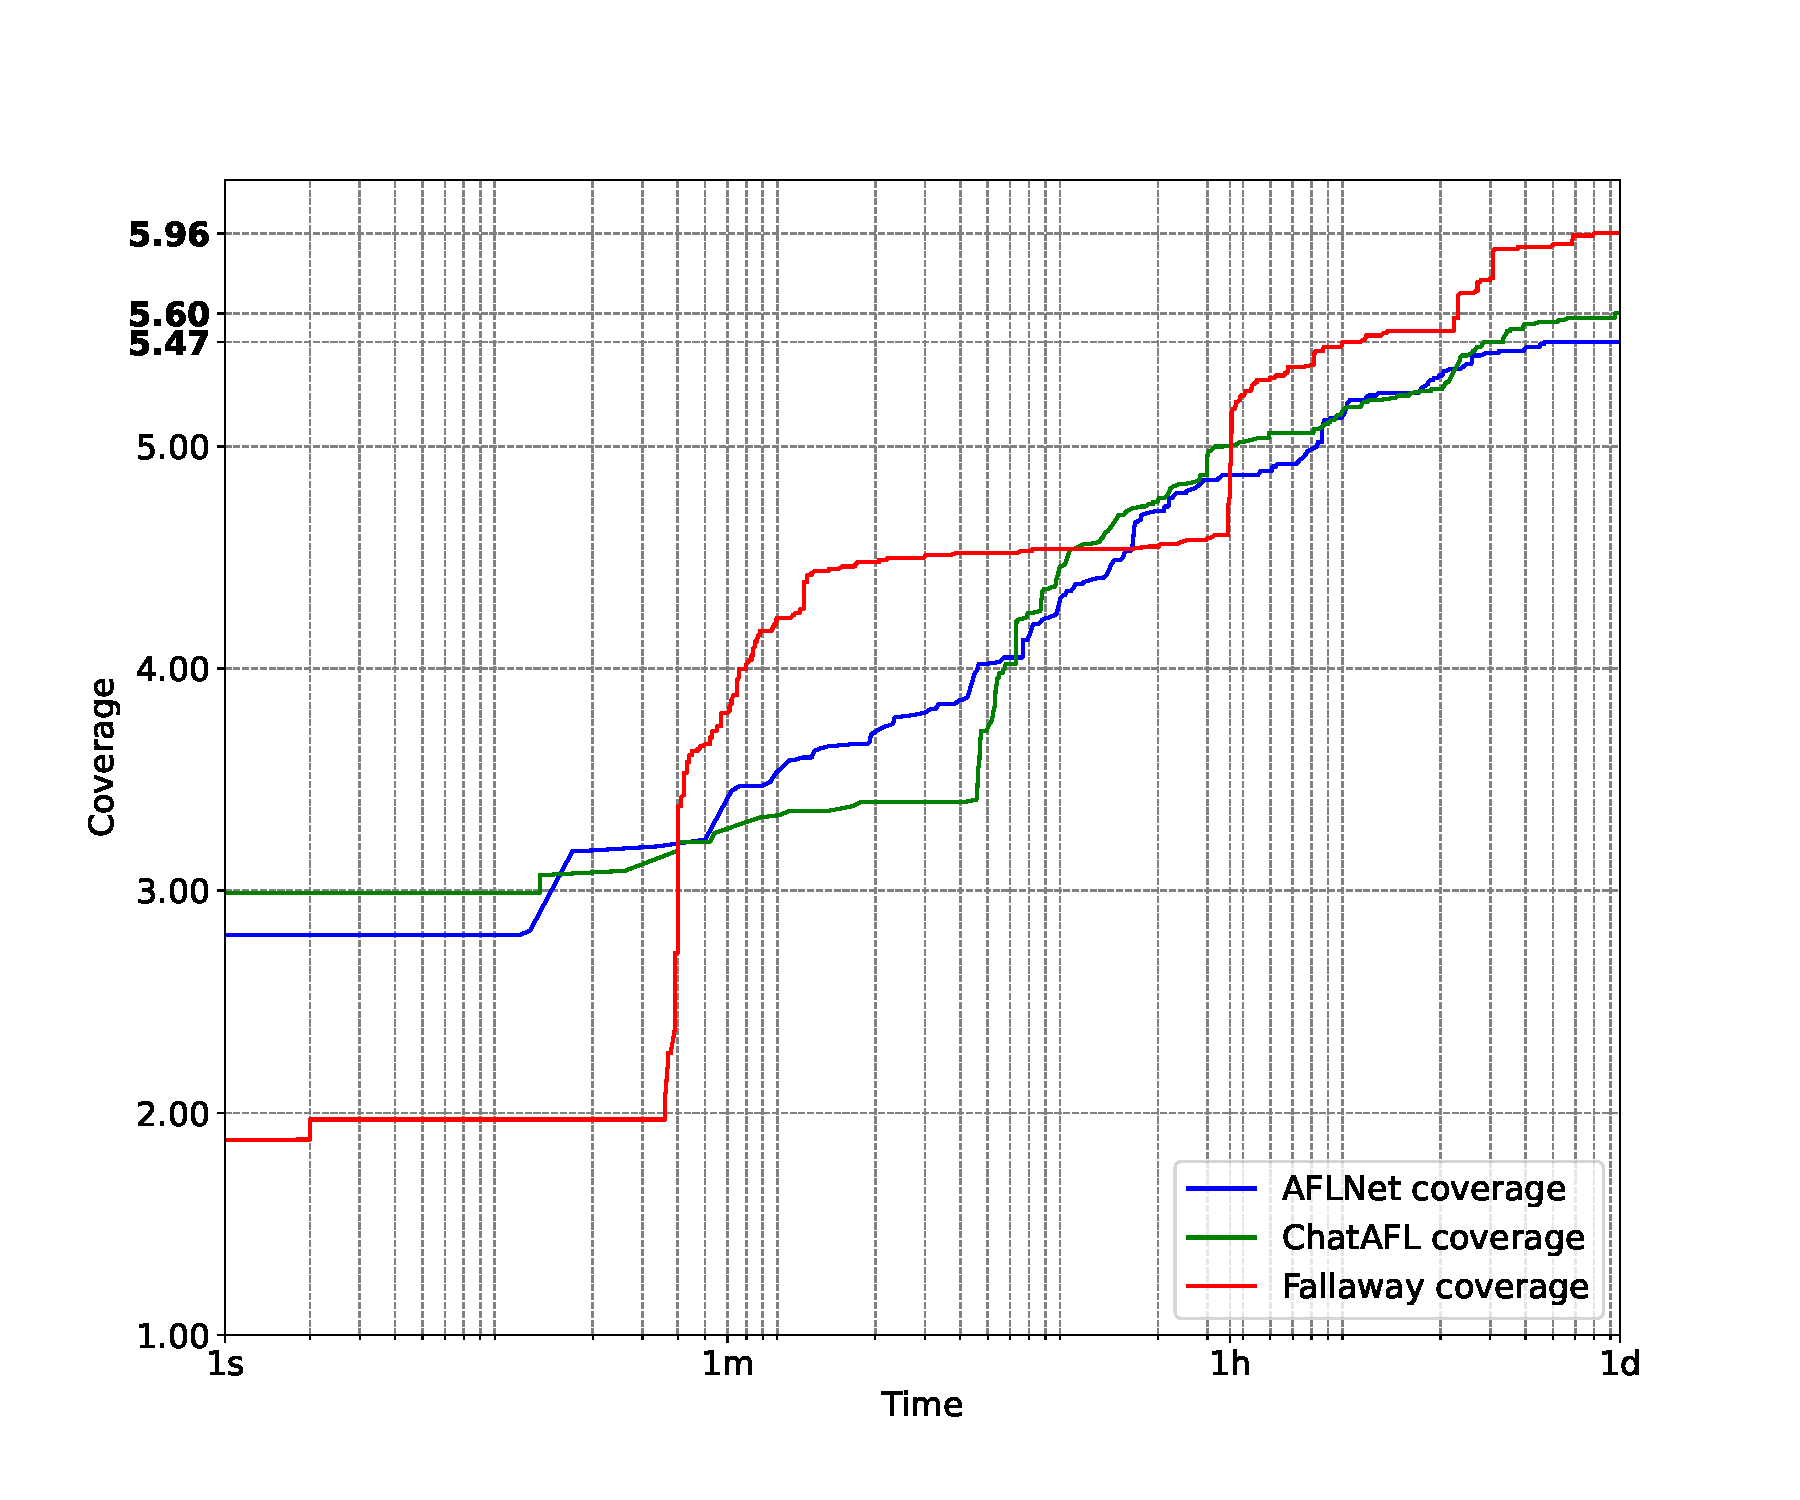
\includegraphics[width=1\textwidth]{Images/coverage_over_time_lighttpd-1day-2000l.pdf}
    \caption{Coverage of the three fuzzers in 24h with Fallaway in a loop of 2000}
    \label{fig:coverage_1day_2000l}
\end{figure}

\begin{figure}[H]
    \centering
    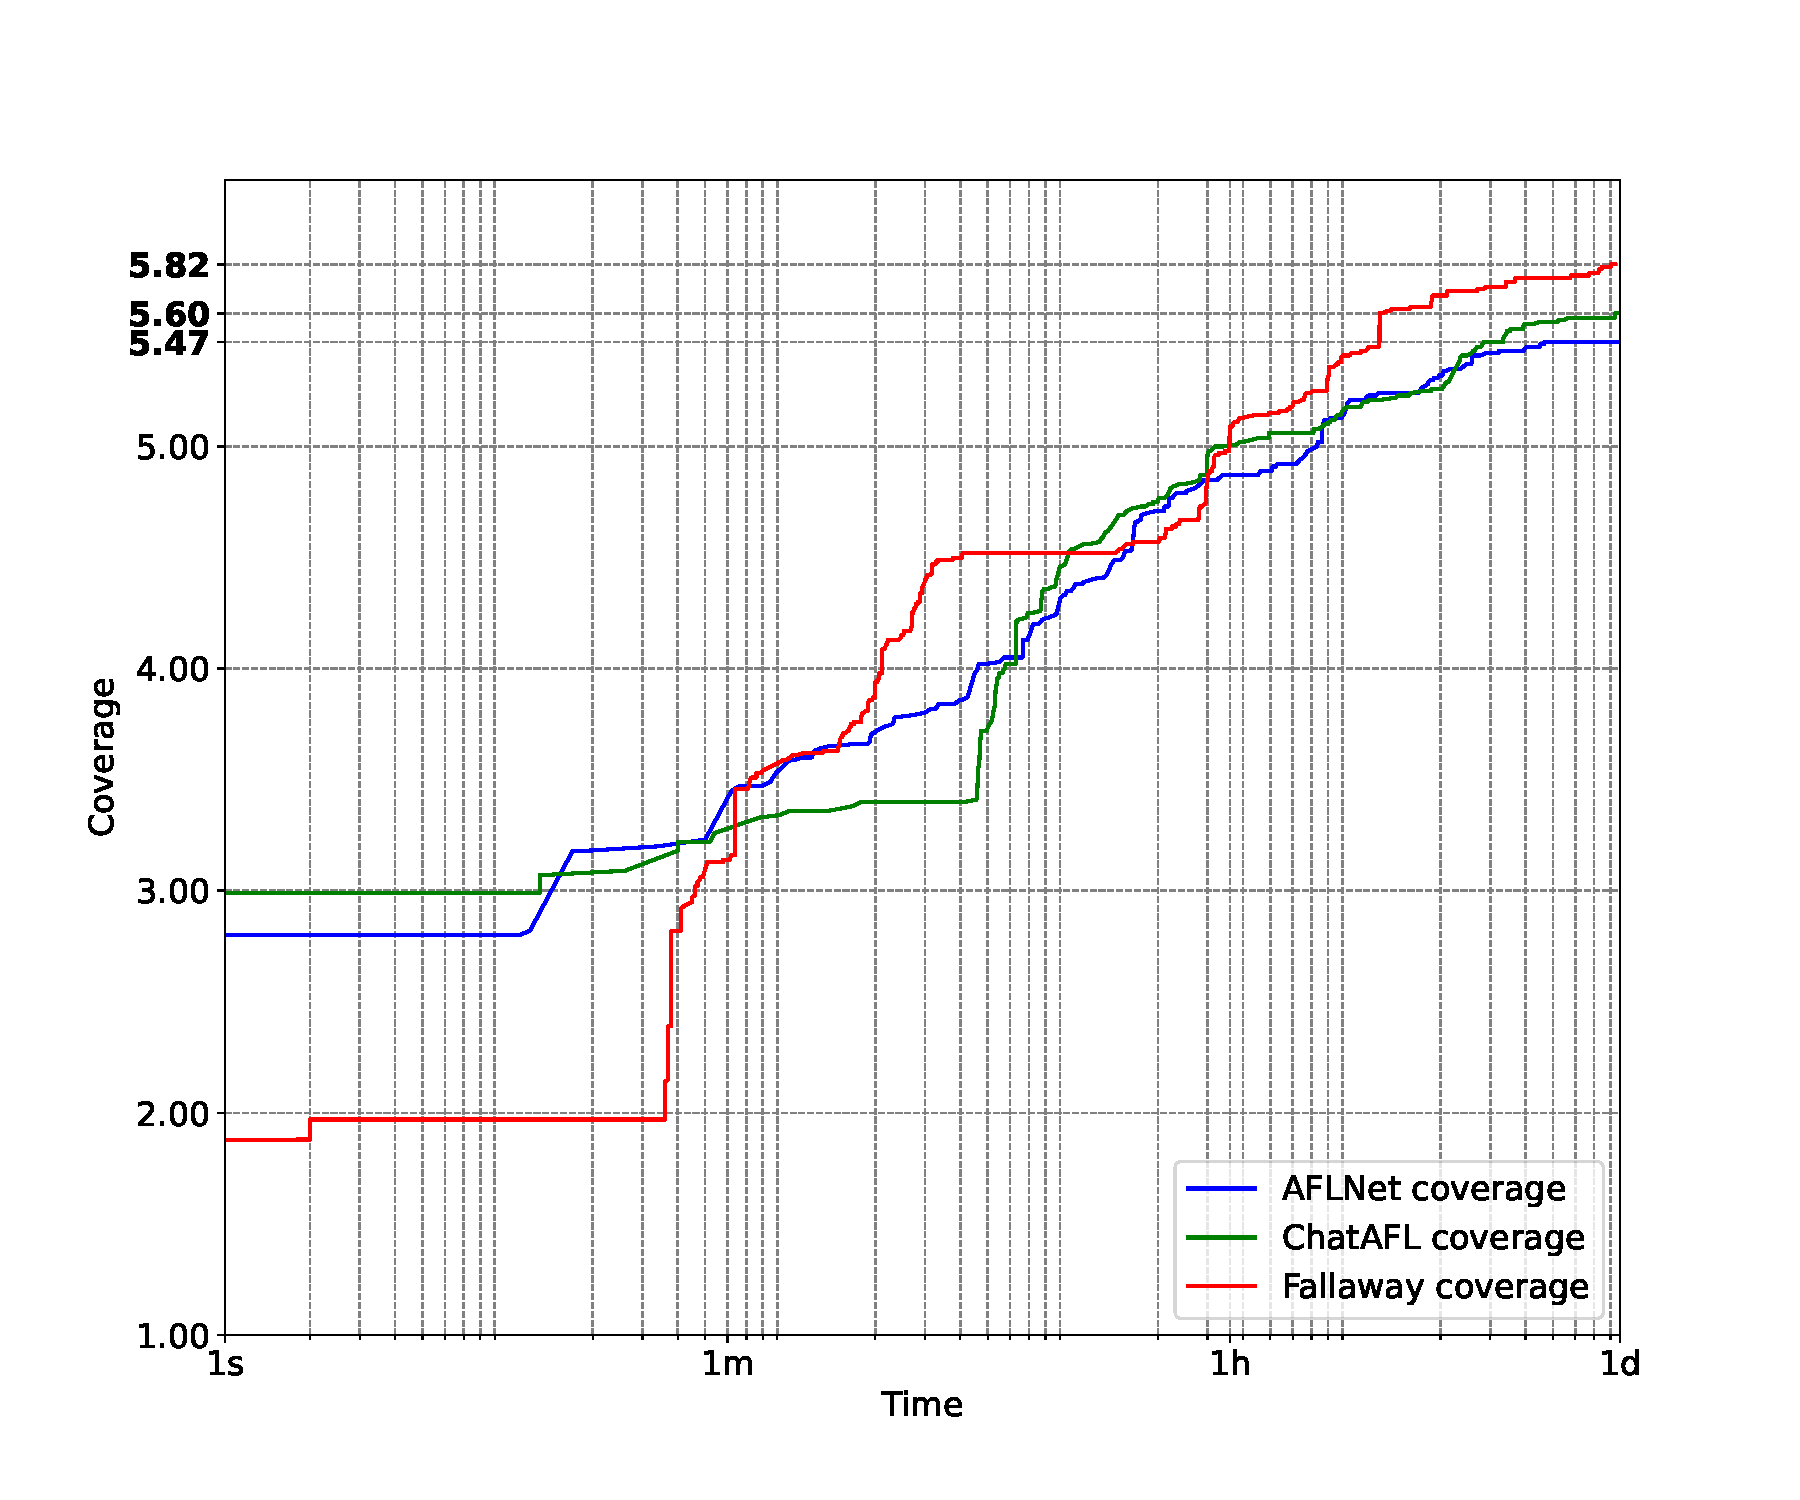
\includegraphics[width=1\textwidth]{Images/coverage_over_time_lighttpd-1day-1000l.pdf}
    \caption{Coverage of the three fuzzers in 24h with Fallaway in a loop of 1000}
    \label{fig:coverage_1day_1000l}
\end{figure}

\begin{figure}[H]
    \centering
    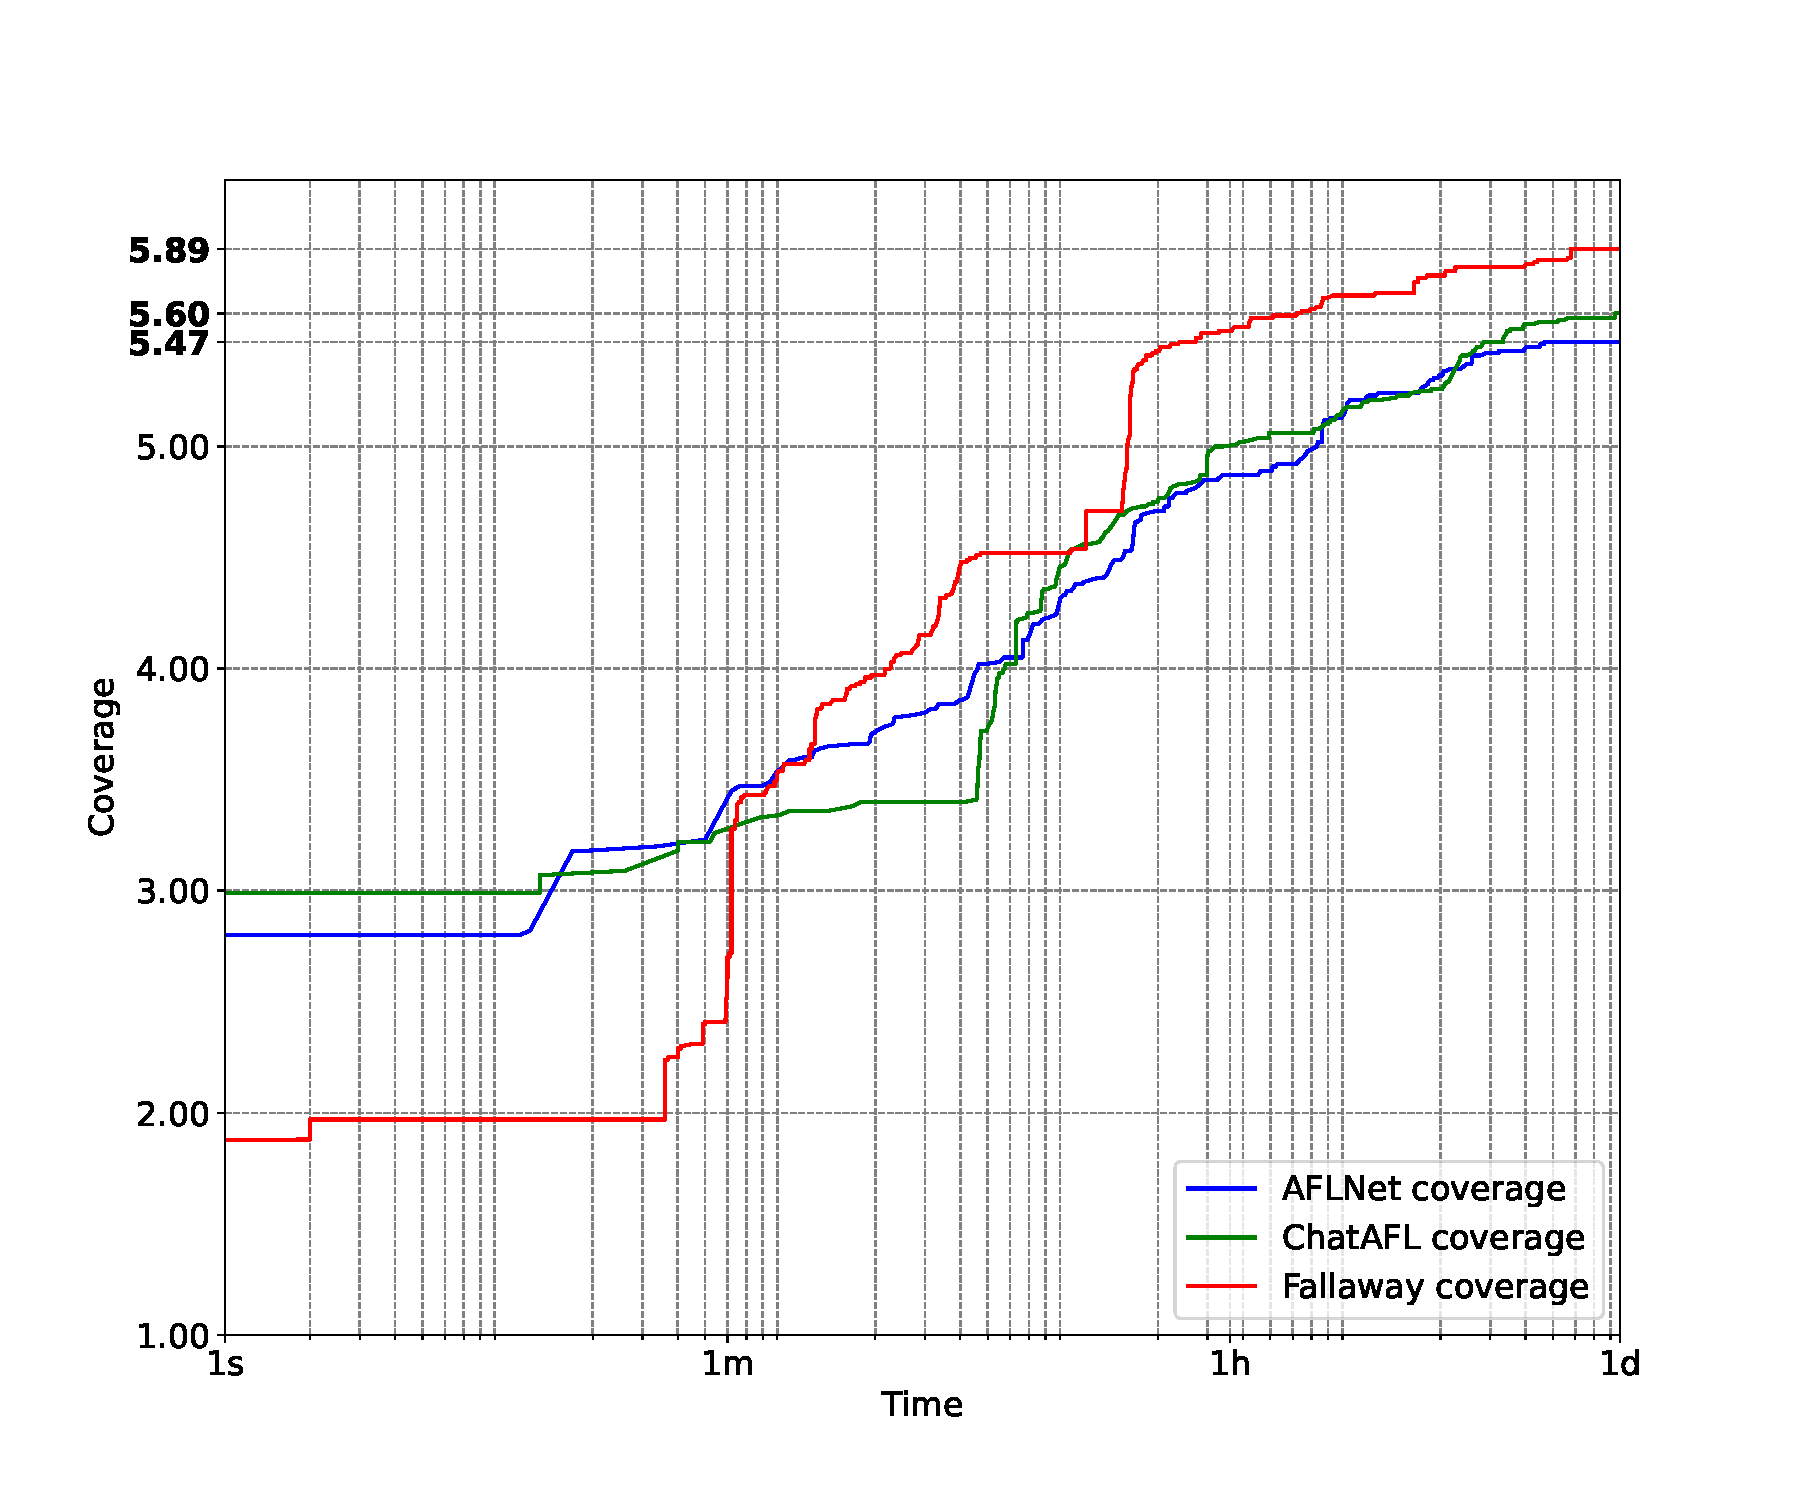
\includegraphics[width=1\textwidth]{Images/coverage_over_time_lighttpd-1day-500l.pdf}
    \caption{Coverage of the three fuzzers in 24h with Fallaway in a loop of 500}
    \label{fig:coverage_1day_500l}
\end{figure}

\begin{figure}[H]
    \centering
    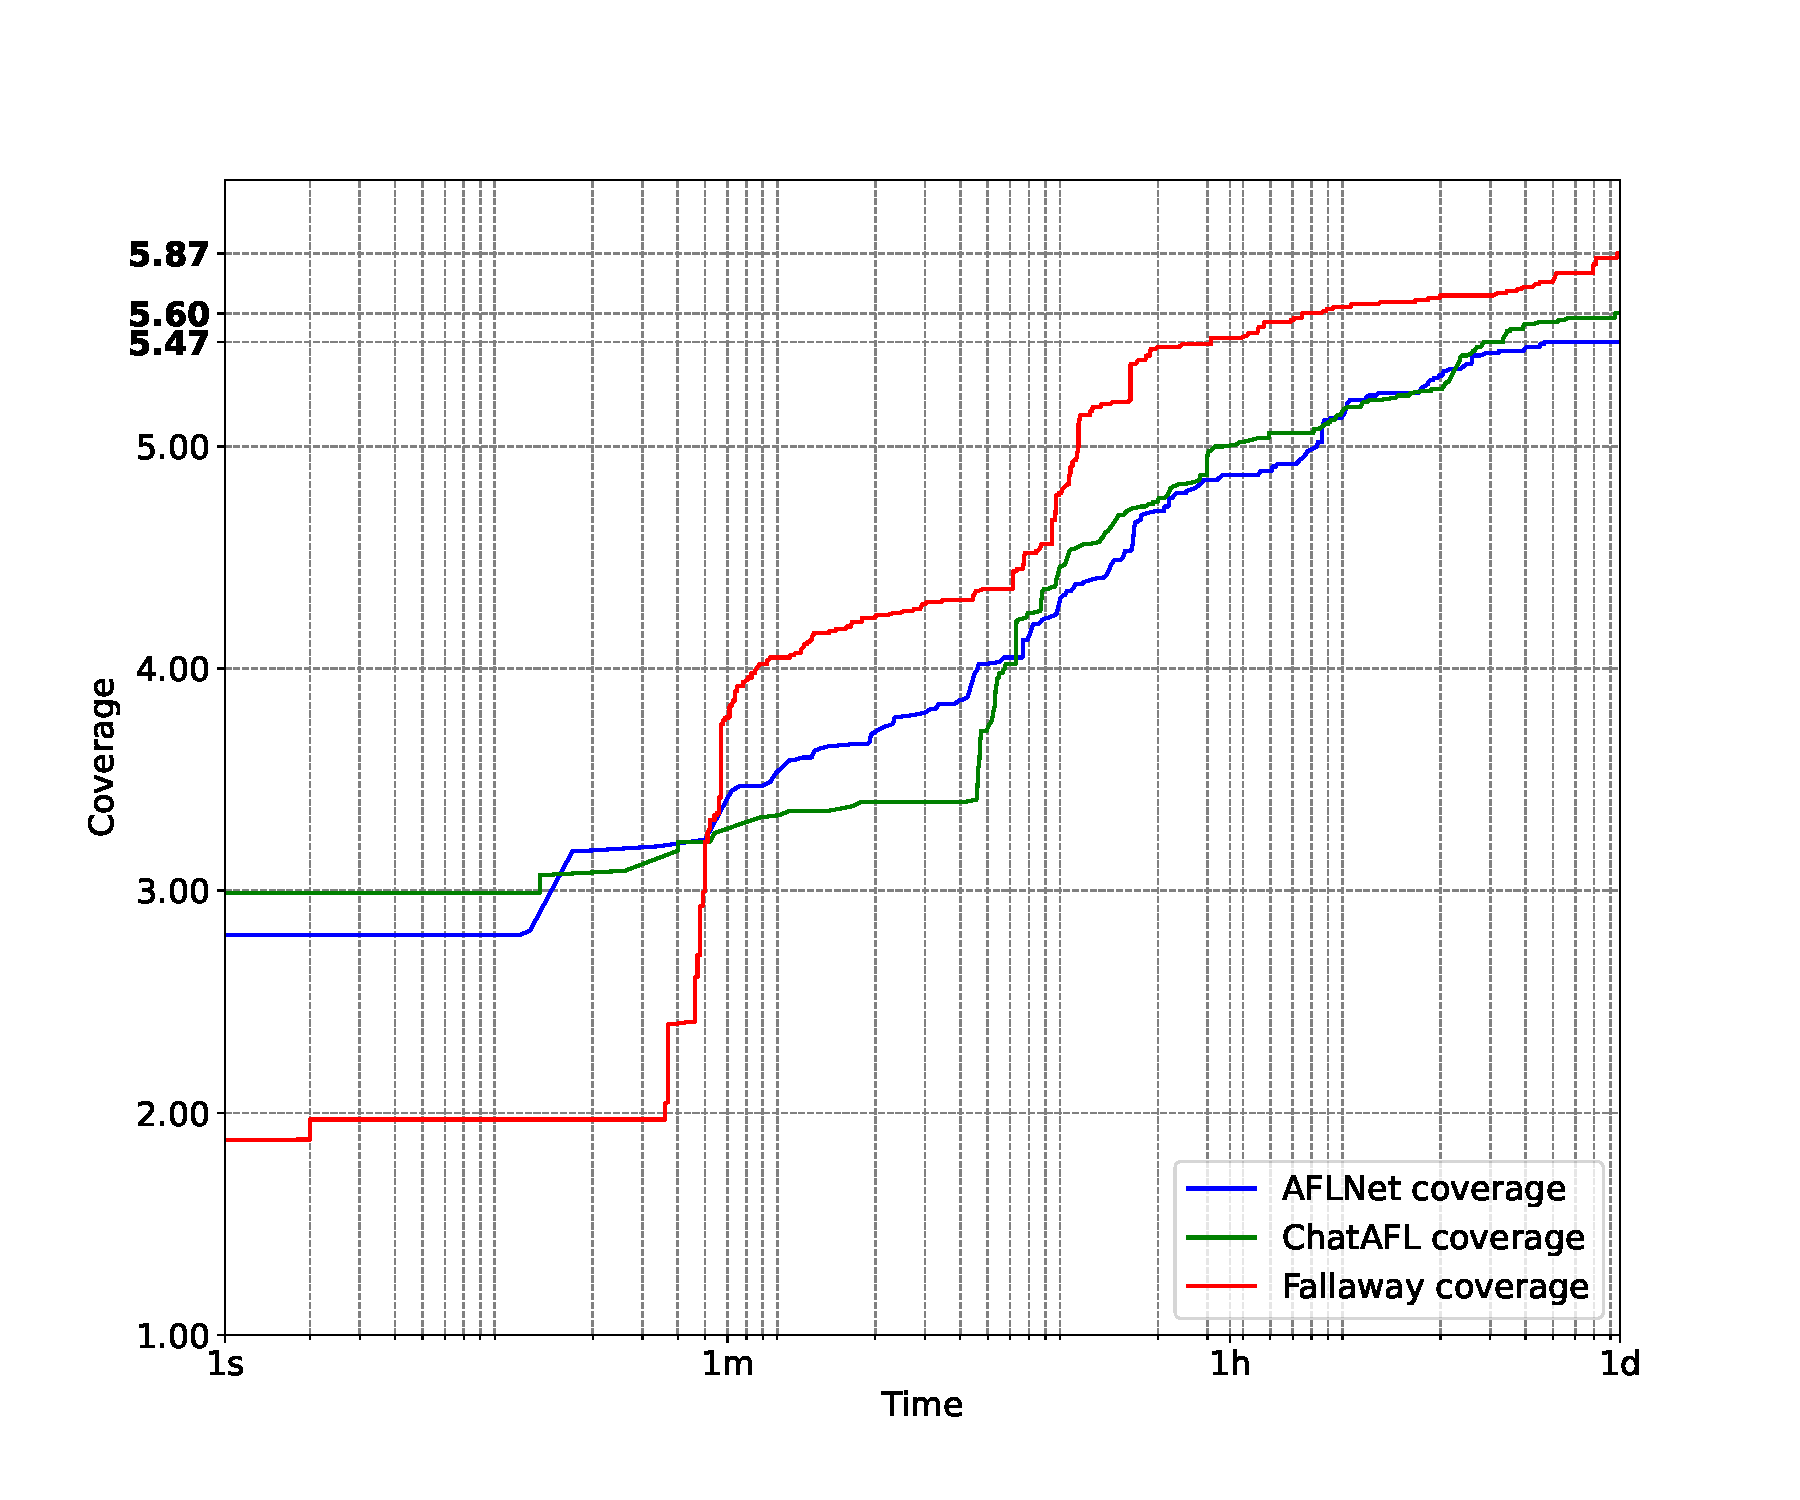
\includegraphics[width=1\textwidth]{Images/coverage_over_time_lighttpd-1day-250l.pdf}
    \caption{Coverage of the three fuzzers in 24h with Fallaway in a loop of 250}
    \label{fig:coverage_1day_250l}
\end{figure}

\begin{figure}[H]
    \centering
    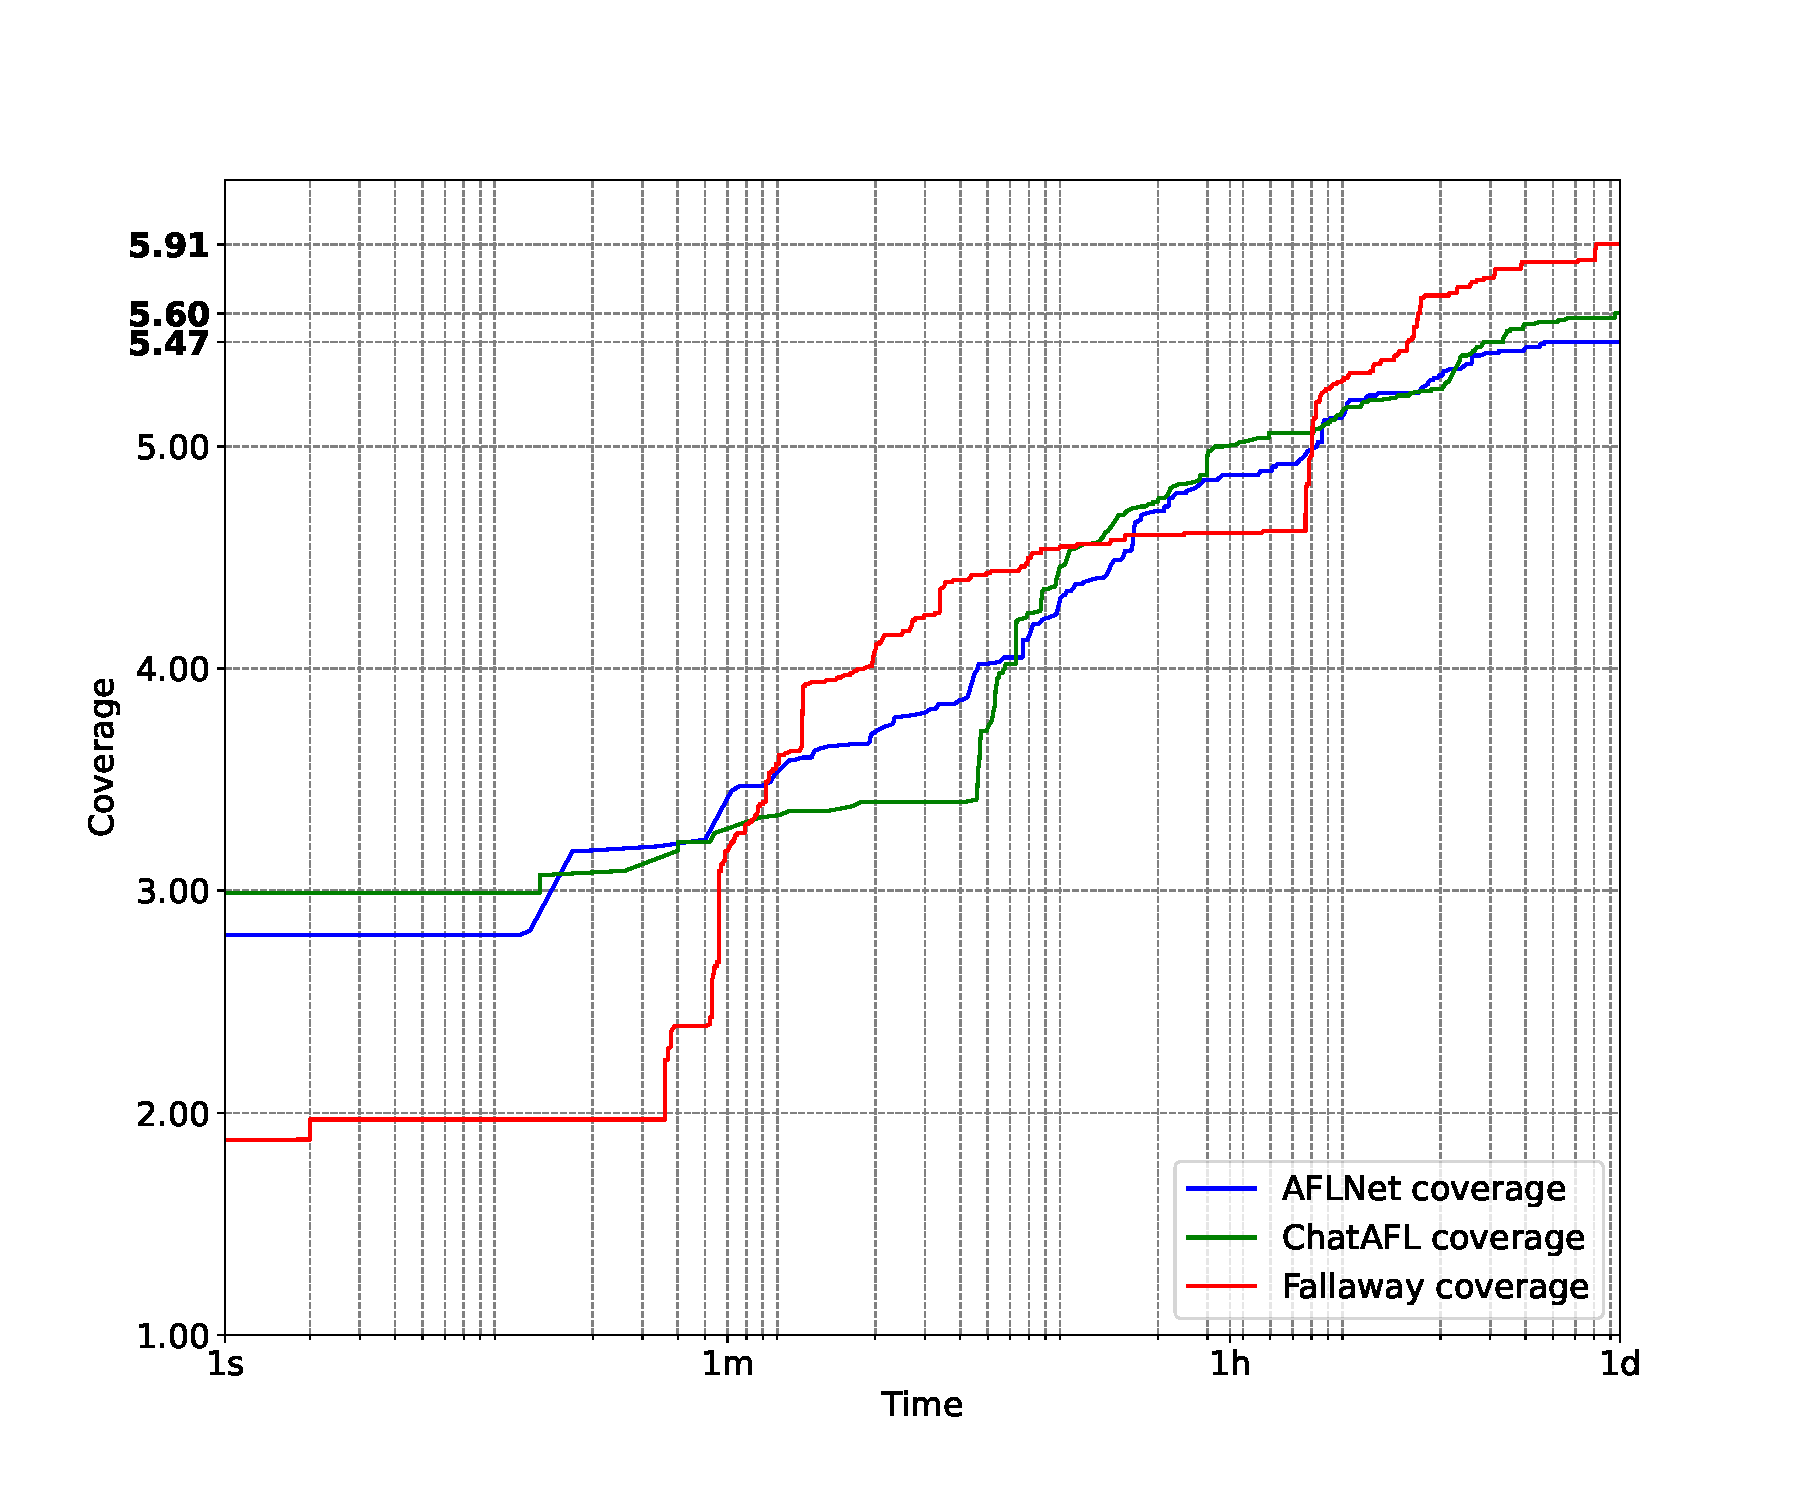
\includegraphics[width=1\textwidth]{Images/coverage_over_time_lighttpd-1day-100l.pdf}
    \caption{Coverage of the three fuzzers in 24h with Fallaway in a loop of 100}
    \label{fig:coverage_1day_100l}
\end{figure}

\begin{figure}[H]
    \centering
    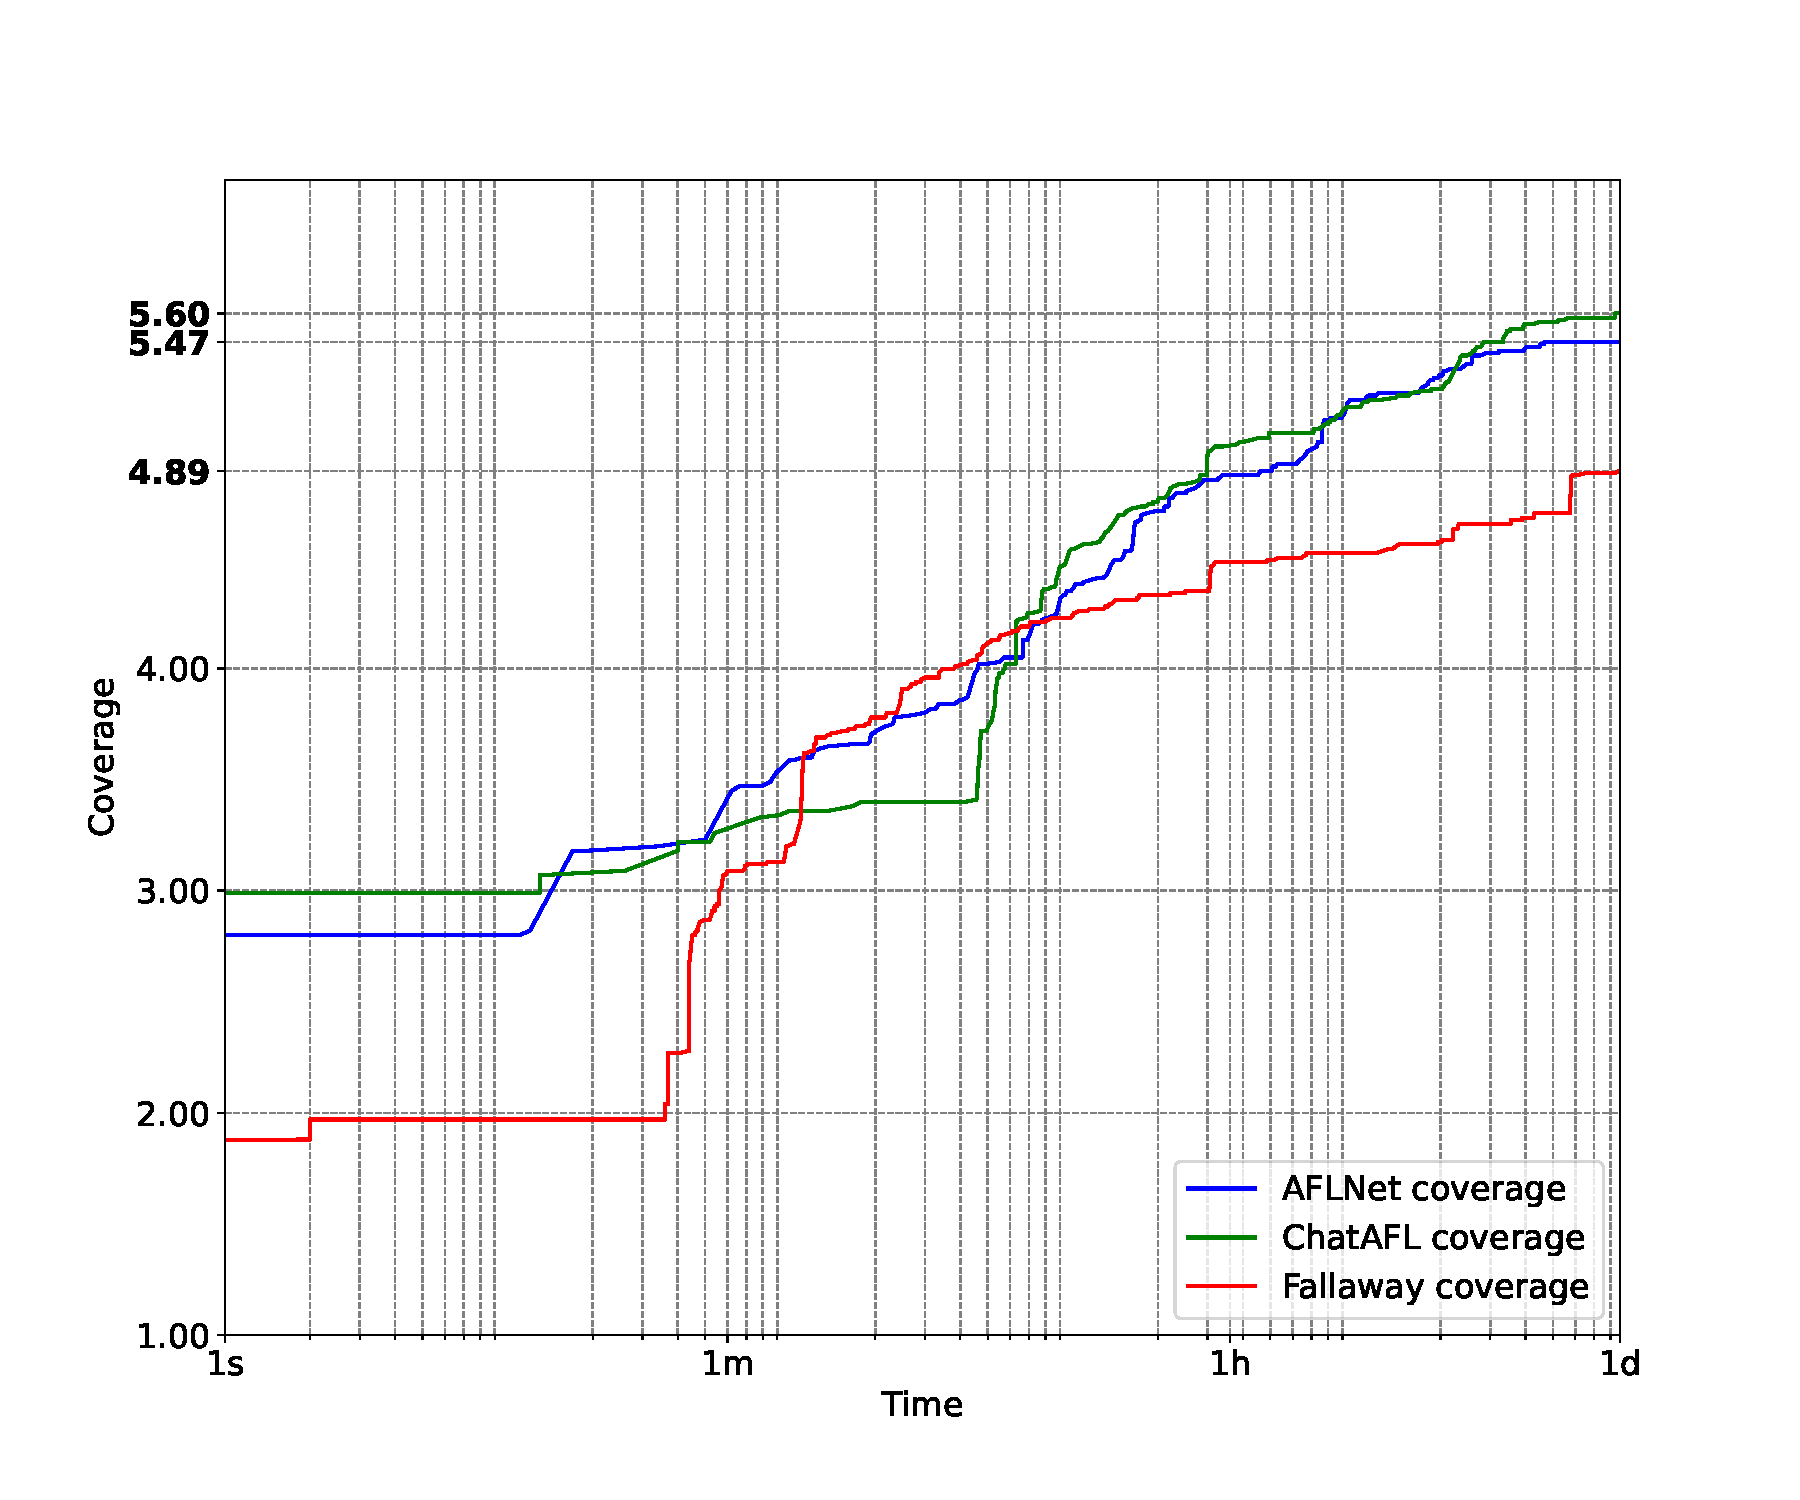
\includegraphics[width=1\textwidth]{Images/coverage_over_time_lighttpd-1day-10l.pdf}
    \caption{Coverage of the three fuzzers in 24h with Fallaway in a loop of 10}
    \label{fig:coverage_1day_10l}
\end{figure}

\begin{figure}[H]
    \centering
    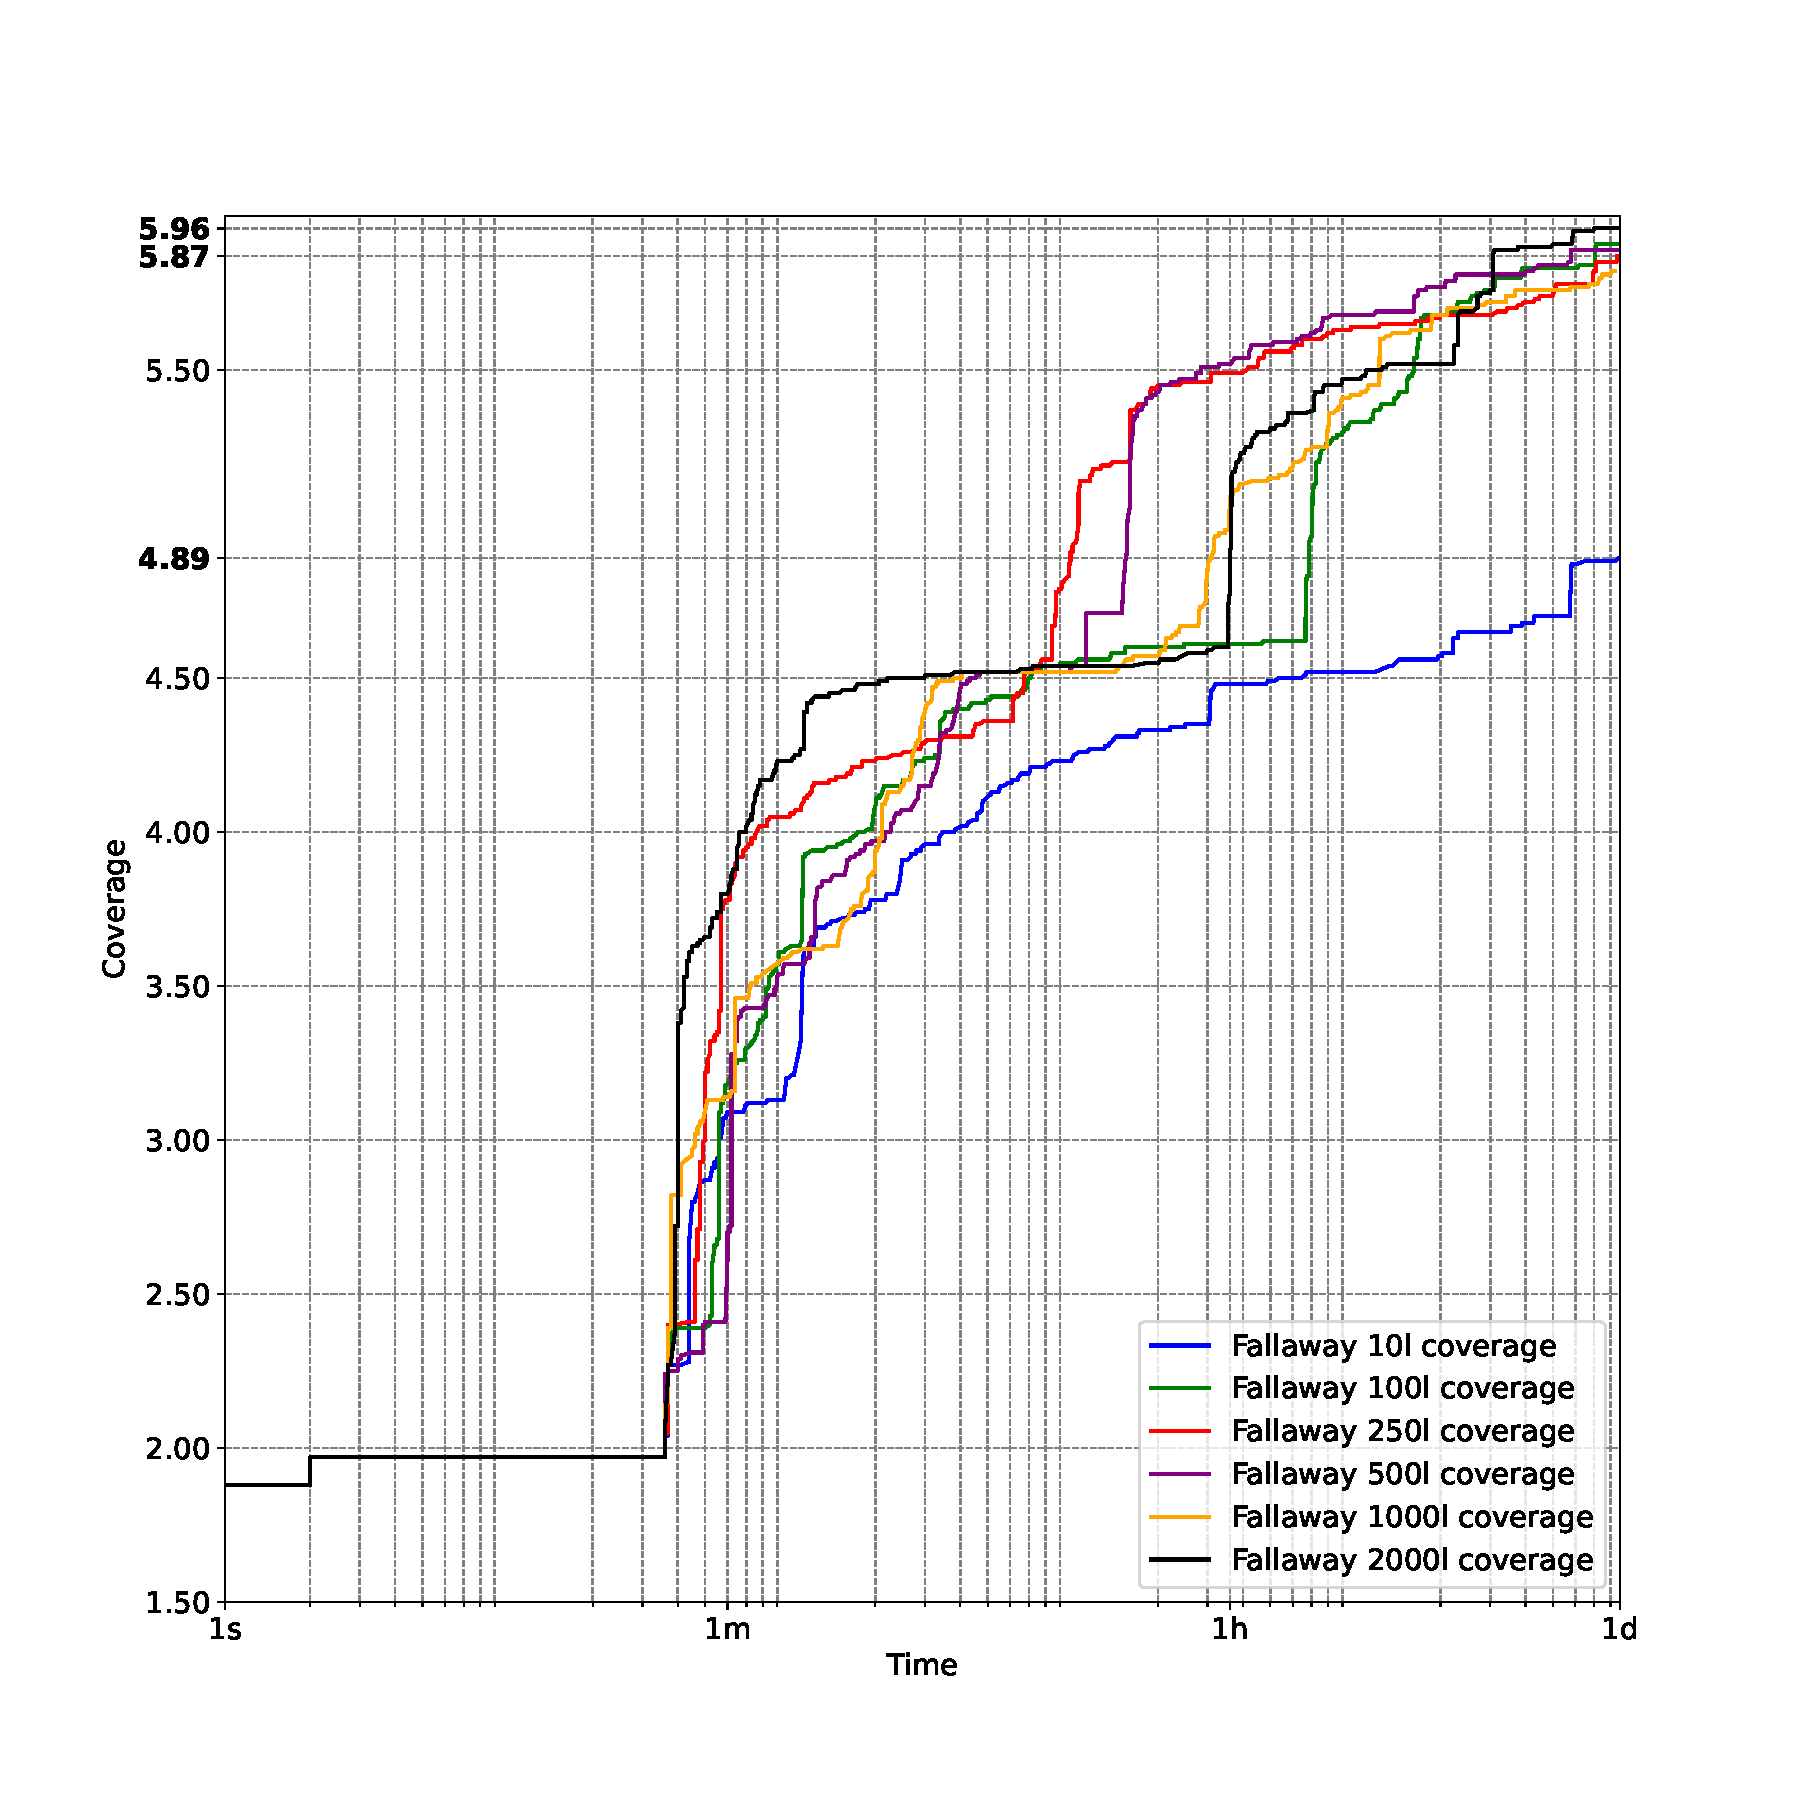
\includegraphics[width=1\textwidth]{Images/coverage_over_time_lighttpd-1day-fallaways.pdf}
    \caption{Coverage of Fallaway's differents configurations in 24h}
    \label{fig:coverage_1day_fallaways}
\end{figure}
\phantom{}\\
As shown in Figure \ref{fig:coverage_1day_2000l}, Fallaway with a loop count of 2000 achieves the highest coverage. This is likely because the fuzzer can execute more test cases before transitioning between states. The other configurations of Fallaway, except for the one with 10 loops, share a lower coverage than the 2000 loops' case, having an average coverage of 5.87\%.
\\Although the loop counts differ, the coverage does not change significantly. This may be due to the implemented state model, which only considers two states: the existence or non-existence of a resource. As a result, even if the number of loops — and thus the number of possible test cases before changing states — varies, the coverage remains relatively stable. This limitation could be addressed by defining a more refined state model that includes additional states.
\\Figure \ref{fig:coverage_1day_10l} shows the lowest coverage at 4.89\%. In this scenario, the low loop count suggests a minimal number of possible test cases before switching states, which reduces the likelihood of extensive exploration.
\\In general, higher loop values can lead to greater coverage by exploring more states, but they may also cause deadlock states where progress is limited. Conversely, lower loop values can help overcome deadlock states more quickly, but they might not explore certain states in depth.
\\Fallaway does not always exhibit linear growth in coverage; instead, it shows a more random behavior, even though its approach yields the best results observed. In contrast, AFLNet and ChatAFL demonstrate more linear growth in coverage, which indicates greater efficiency in code exploration. They start with higher initial coverage than Fallaway, suggesting they are better at targeting diverse code paths.
\\The linearity is shown using the \textit{Pearson correlation coefficient} in Table \ref{tab:pearson_correlation}.
Pearson correlation coefficient measures the strength and direction of a linear relationship between two variables (in this case, time and coverage). The closer the coefficient is to 1, the stronger the linear relationship is.
In this case, the coefficient for AFLNet and ChatAFL is 0.67, indicating a good linear relationship between time and coverage.
\\Fallaway's coefficient varies, depending on the loop count, with the highest value of 0.71 for 100 loops and the lowest value of 0.47 for 500 loops. This suggests that Fallaway with 100 loops has the most linear relationship between time and coverage, instead of the 500 loops configuration, which has the lowest linear relationship.
\\Regarding coverage, AFLNet achieves a coverage of 5.47\% with significantly fewer executions compared to the closest coverage for Fallaway's configurations (1000 loop, see Table \ref{tab:fuzzer_comparison}).
\\ChatAFL reaches 5.60\% coverage with a number of executions similar to AFLNet. As ChatAFL is based on AFLNet, it effectively surpasses the coverage plateau observed with AFLNet. In particular, as shown in Figure \ref{fig:coverage_1day_10l}, which minimizes the interference from Fallaway, ChatAFL surpasses AFLNet's coverage plateau most of the time. Additionally, within the 1-day timeframe, it exhibits a slight increase in coverage, indicating that it was able to exceed its own previous plateau.
\begin{table}[H]
    \centering
    \begin{tabular}{|c|c|}
    \hline
    \textbf{Fuzzer} & \textbf{Pearson Correlation Coefficient} \\
    \hline
    Fallaway 2000 & 0.67 \\
    \hline
    Fallaway 1000 & 0.64 \\
    \hline
    Fallaway 500 & 0.47 \\
    \hline
    Fallaway 250 & 0.53 \\
    \hline
    Fallaway 100 & 0.71 \\
    \hline
    Fallaway 10 & 0.54 \\
    \hline
    AFLNet & 0.67 \\
    \hline
    ChatAFL & 0.67 \\
    \hline
    \end{tabular}
    \caption{Pearson Correlation Coefficient for the three fuzzers}
    \label{tab:pearson_correlation}
\end{table}

\phantom{}\\

\subsection{Fallaway}
\label{sec:fallaway_analysis}

\textbf{Strengths:}
\begin{itemize}
    \item \textit{Higher Execution Count}: Fallaway has a significantly higher number of total executions compared to AFLNet and ChatAFL, indicating its capability to generate and execute a large number of test cases. This increases the likelihood of discovering bugs or vulnerabilities through extensive input space exploration. An important distinction is that Fallaway treats each execution as a single input, whereas AFLNet and ChatAFL treat executions as full \textit{traces}—sequences of inputs, typically 5 or 6, sent before restarting the SUT's process. Therefore, the adjusted number of executions for a fair comparison with Fallaway is 1,258,656 for AFLNet and 1,447,452 for ChatAFL. Even with this adjustment, Fallaway still has a higher number of executions.
    \item \textit{Higher Code Coverage}: Achieves the highest code coverage among the three fuzzers (5.96\%), suggesting its strategy, even if may lacks of  sophistication in targeting specific code paths relies on brute force to uncover edge cases, is effective at exploring various parts of the code.
\end{itemize}

\textbf{Weaknesses:}
\begin{itemize}
    \item \textit{Efficiency Concerns}: The large number of total executions (nearly 120 million in the best case) suggests that Fallaway may be less efficient, requiring more attempts to cover similar amounts of code compared to AFLNet and ChatAFL.
\end{itemize}


\subsection{AFLNet}

\textbf{Strengths:}
\begin{itemize}
    \item \textit{Efficient Execution}: With the lowest number of total executions (around 210,000), AFLNet is highly efficient in achieving its results. This suggests AFLNet is effective in targeting specific code parts with minimal test cases, leveraging coverage-guided strategies.
\end{itemize}

\textbf{Weaknesses:}
\begin{itemize}
    \item \textit{Lower Code Coverage}: AFLNet achieves slightly lower coverage (5.47\%) compared to Fallaway and ChatAFL, indicating it might not explore as many diverse code paths outside of network protocol contexts.
\end{itemize}

\subsection{ChatAFL}

\textbf{Strengths:}
\begin{itemize}
    \item \textit{Balanced Approach}: ChatAFL exhibits a balance between execution count and coverage. With a small number of executions (around 241,000) and a good code coverage (5.60\%), it balances efficiency and effectiveness.
\end{itemize}

\textbf{Weaknesses:}
\begin{itemize}
    \item \textit{Potential Limitations in General Fuzzing Tasks}: While optimized for certain scenarios, its overall effectiveness may vary depending on the specific use case and target application. Even though it performs many more state changes \cite{chatafl}, it does not achieve a significant increase in coverage in this case study.
\end{itemize}